\documentclass{article}
\usepackage{amsmath,graphicx}

\begin{document}
\title{SLAM}
\date{}
\maketitle

\section{Introduction}

The problem of planar mobile robot mapping is to estimate a 2D map of world using a mobile robot equipped with odometry and sensors.  A map of the world allows a robot to perform accurate localization and efficient path planning.  Both of these are key problems for any mobile robot performing useful tasks in an environment such as vacuuming floors.

Robot perception of the world is imperfect because of noise in sensor readings.  Moreover, there is also an accumulation of errors in odometry as a robot moves over time.  Both of these issues are problematic for mapping because each causes errors in mapping, and it seems difficult to solve both at the same time.  In fact, most of the earlier work in robot mapping, simplified the formulation by essentially assuming known robot pose and focused on fusing noisy measurements.

More recent work in simultaneous localization and mapping (SLAM) exploits the fact that robot odometry generates systematic errors (because of accumulation), while measurement errors are random, so that the estimated map error is correlated with robot path error.  This allows a joint formulation of the robot mapping and localization problem.  The formulation is principled and consistent, so that most of the work is focused on practical approximations to intractable computations.

\section{SLAM}

The SLAM problem is to estimate the probability distribution of the robot path and the world map:
\begin{equation}
p(s_t, M | z_{1:t}, u_{1:t}),
\end{equation}
where $s_t$ is the state of the robot at time $t$, $M$ is the map, and $z_{1:t}$ and $u_{1:t}$ are the robot sensor measurements and controls, respectively, over time.  The idea behind a probabilistic model is so that not only can an expected robot pose and world map be calculated, but also the uncertainty in these variables, as well as any other statistics.  If it is assumed that the robot path is known, then estimating the world map is considerably easier---this is the subject of much earlier robot mapping work before SLAM became popular.

A solution to the SLAM problem is the recursive Bayes filter:
\begin{equation}
p(s_t, M | z_{1:t}, u_{1:t}) = \frac{1}{A} p(z_t | s_t, M) \int p(s_t|s_{t-1},u_t) p(s_{t-1}, M | z_{1:t-1}, u_{1:t-1}) ds_{t-1}.
\label{eqn:bayes}
\end{equation}
The first term on the right-hand side is a normalization constant to ensure that the left-hand side is a proper probability distribution.  The second term on the right-hand side is the measurement model.  It models the robot sensor readings given the robot state and world map.  The first term in the integral is the robot motion model.  It models the robot control and odometry.  The filter factors the current probability distribution into a product of the current measurement distribution and an integral over the previous probability distribution and the robot motion model.  This allows recursive updates to the probability distribution given the previous one over time.

Although equation \ref{eqn:bayes} is mathematically simple, computing the integral is usually intractable unless the state space is finite or the probability distributions allow analytic calculations, such as for the case of Gaussians.  In summary, the recursive Bayes filter requires three components: 1. a measurement model $p(z_t | s_t, M)$, 2. a state transition distribution $p(s_t|s_{t-1},u_t)$, and 3. an initial probability distribution $p(s_0, M)$.

\subsection{FastSLAM}

Early approaches to SLAM used the Extended Kalman Filter (EKF) approach to jointly estimate robot pose and world map.  Although effective, these approaches require quadratic, in the number of landmarks in the map, memory and computation.  This stems from the quadratic nature of the covariance matrix in multi-variate Gaussian distributions.

The FastSLAM method takes advantage of the factorization of the distribution of landmarks given the robot path:
\begin{equation}
p(s_{1:t}, M | z_{1:t}, u_{1:t}) = p(s_{1:t}, | z_{1:t}, u_{1:t}) \prod_i p(f_i | s_{1:t}, z_{1:t}, u_{1:t}),
\end{equation}
where $s_{1:t}$ is the robot path (instead of just pose $s_t$) and $f_i$ are landmarks in the world map.  As is often the case in practical algorithms for Bayesian estimation, the idea here is to factorize a complicated probability distribution into a product of simpler ones.  This formulation avoids explicit modeling of the correlation between landmarks as was done in EKF SLAM.  The method uses a particle filter to model the robot path and $n$ independent EKFs to model the landmarks.  This avoids the quadratic memory and computation requirements of EKF SLAM.

\subsection{GraphSLAM}

One particular clean and generic formulation of the SLAM problem is GraphSLAM.  It tackles the full SLAM problem:
\begin{equation}
p(s_{1:t}, M | z_{1:t}, u_{1:t}),
\end{equation}
which solves for the full robot pose given the entire temporal history of controls and measurements.  The formulation represents robot poses and elements in the world map as nodes in a graph with edges corresponding to relations between poses, induced by the control, and relations between poses and measurements induced by the sensing.  Given the entire graph the values of the nodes are optimized to best satisfy the relations.  The graph is usually sparse and other techniques are used to make the computation tractable.  Indeed, this global joint optimization accounts for much of the power of GraphSLAM for a given fixed-sized batch of data.

The GraphSLAM cost function is a sum of pairwise terms based on the edges of the graph:
\begin{equation}
E = \sum_t [s_t - g(u_t, s_{t-1})]^T R_t^{-1} [s_t - g(u_t, s_{t-1})] + \sum_t \sum_i [z_{i, t} - h(s_t, M)]^T Q_t^{-1} [z_{i, t} - h(s_t, M)].
\end{equation}
To solve for the robot pose and world map to minimize the cost, GraphSLAM can first initialize values based only on odometry.  It then linearizes the relations between nodes for tractable computation.  Furthermore it can also reduce the graph to one with only robot pose nodes by updating the relation between nodes which observe the same part of the map.  Finally an optimization procedure is run to minimize the cost.  This entire procedure can be iterated with the latest result to improve the estimation.

For the very simple case of a robot with linear motion and sensing, GraphSLAM can be solved as a linear system where the variables consists of the robot poses and map and the matrix captures the pairwise costs between two poses and a pose and a landmark in the map.  This can be seen by observing that the cost function becomes a sum of quadratic terms in the unknowns which can be solved by least squares.  Indeed this is similar to the inner computation of the general GraphSLAM algorithm after linearization.  Figure \ref{fig:graphslamlinear} shows an example of this linear GraphSLAM for a planar mobile robot building a map of world landmarks.  As expected, SLAM significantly improves the odometry estimate of the robot path and gives a reasonable accurate map of the landmarks.  Although the landmarks are helpful in constraining the graph, note that the robot pose nodes form a chain based on time, even when the robot returns to a previously visited location.  However, this should induce constraining edges between the previous nodes and the current pose.  This problem is known as loop closure and approaches for dealing this situation can significantly improve SLAM results.  An illustration of this problem can be seen in Figure  \ref{fig:graphslamlinear} where the final SLAM pose of the robot near the bottom-middle of the plot is off of the true path.

\begin{figure}
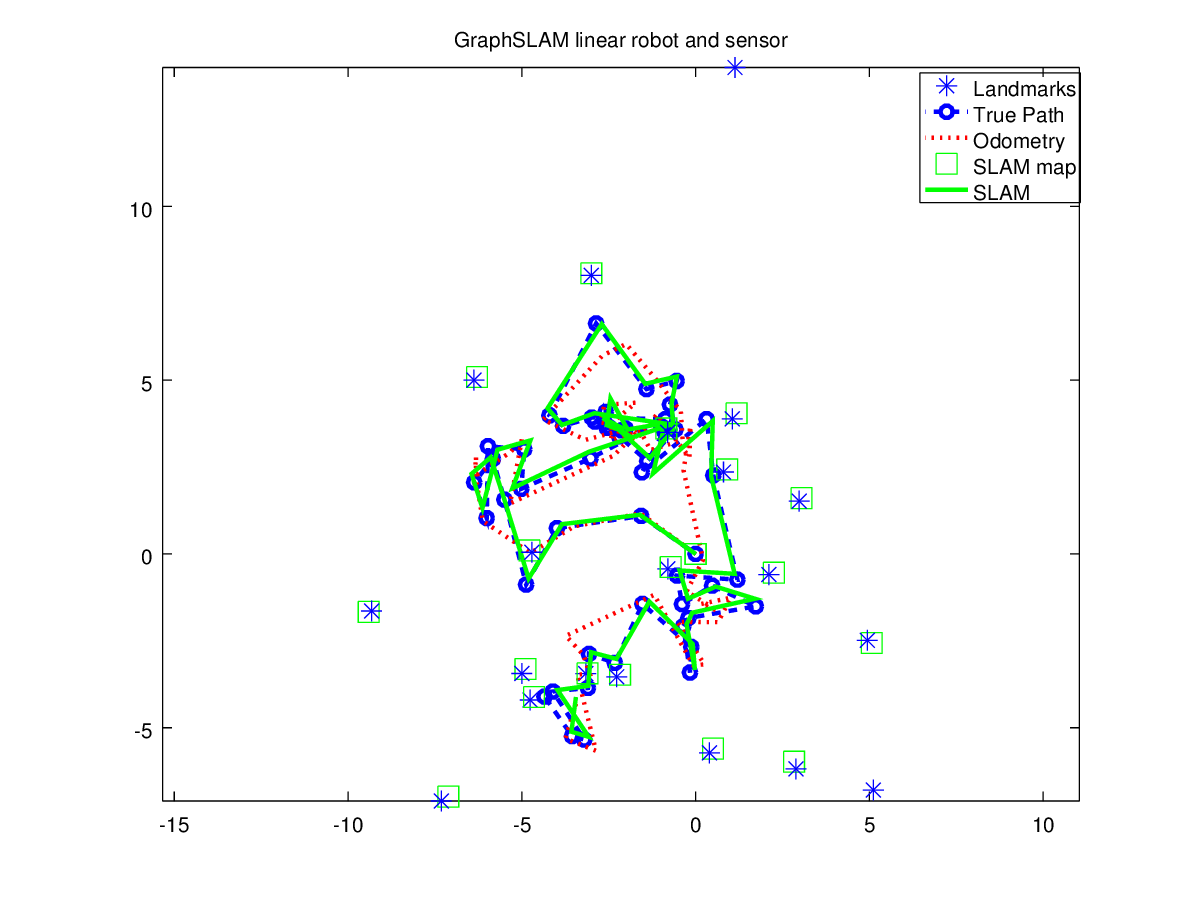
\includegraphics[width=\linewidth]{graphslam/graphslamlinear.png}
\caption{An example of GraphSLAM for a linear robot and sensor.  The true landmarks and path are shown as blue asterisks and dashed blue curve, respectively.  The red dashed curve is the drifted path when using odometry alone.  The green squares and curve are the GraphSLAM estimated map and robot path, respectively.}
\label{fig:graphslamlinear}
\end{figure}

\section{Occupancy Grids}

Early work in robot mapping focused on the mapping problem, assuming that the robot pose is known.  A popular approach is the occupancy grid which represents a map as a discrete grid where the state of each cell is binary, i.e., occupied or empty.  The probability distribution to estimate is,
\begin{equation}
p(M | z_{1:t}, s_{1:t}),
\end{equation}
with cell $m_i \in M$.  As before because $M$ is very high-dimensional, an approximation must be made to enable tractable computation:
\begin{equation}
p(M | z_{1:t}, s_{1:t}) = \prod_i p(m_i | z_{1:t}, s_{1:t})
\end{equation}

The occupancy grid model involves mainly keeping track of the log odds of occupancy for each cell:
\begin{equation}
L_{i, t} =\log \frac{p(m_i=1|z_{1:t}, x_{1:t})}{p(m_i=0|z_{1:t}, x_{1:t})} = \log \frac{p(m_i=1|z_{1:t}, x_{1:t})}{1 - p(m_i=1|z_{1:t}, x_{1:t})}. 
\end{equation}
The update equation is
\begin{equation}
L_{i, t} = L_{i, t-1} +  \log \frac{p(m_i=1|z_{1:t}, x_{1:t})}{1 - p(m_i=1|z_{1:t}, x_{1:t})}  - L_0,
\end{equation}
where
\begin{equation}
L_0 = \log\frac{p(m_i=1 | s_{1:t})}{p(m_i=0 | s_{1:t})}
\end{equation}
is the prior probability of occupancy.  Cells outside of the sensor field-of-view are not updated.  The values for the log odds depends on the particular sensor and cell.  For example, with a range sensor, cells near the measured range are likely to be occupied so the log odds would be positive, while cells between the range and the robot are likely to be empty so the log odds would be negative, etc.  Basically the occupancy grid integrates evidence from the sensor over time regarding each cell's probability of occupancy.

Although the assumption of known robot pose limits the power of occupancy grids, they do represent the map in a form which is convenient for other tasks such as navigation.  One way to use occupancy grids is to apply them after a SLAM algorithm has successfully estimated the robot pose.  Finally, occupancy grids are simple and efficient to estimate.

Figure \ref{fig:occupgrid} shows a run of a very simple example of occupancy grids for a 1D robot with a range sensor moving towards a wall very similar to the example in Section \ref{sec:kalman}.

\begin{figure}
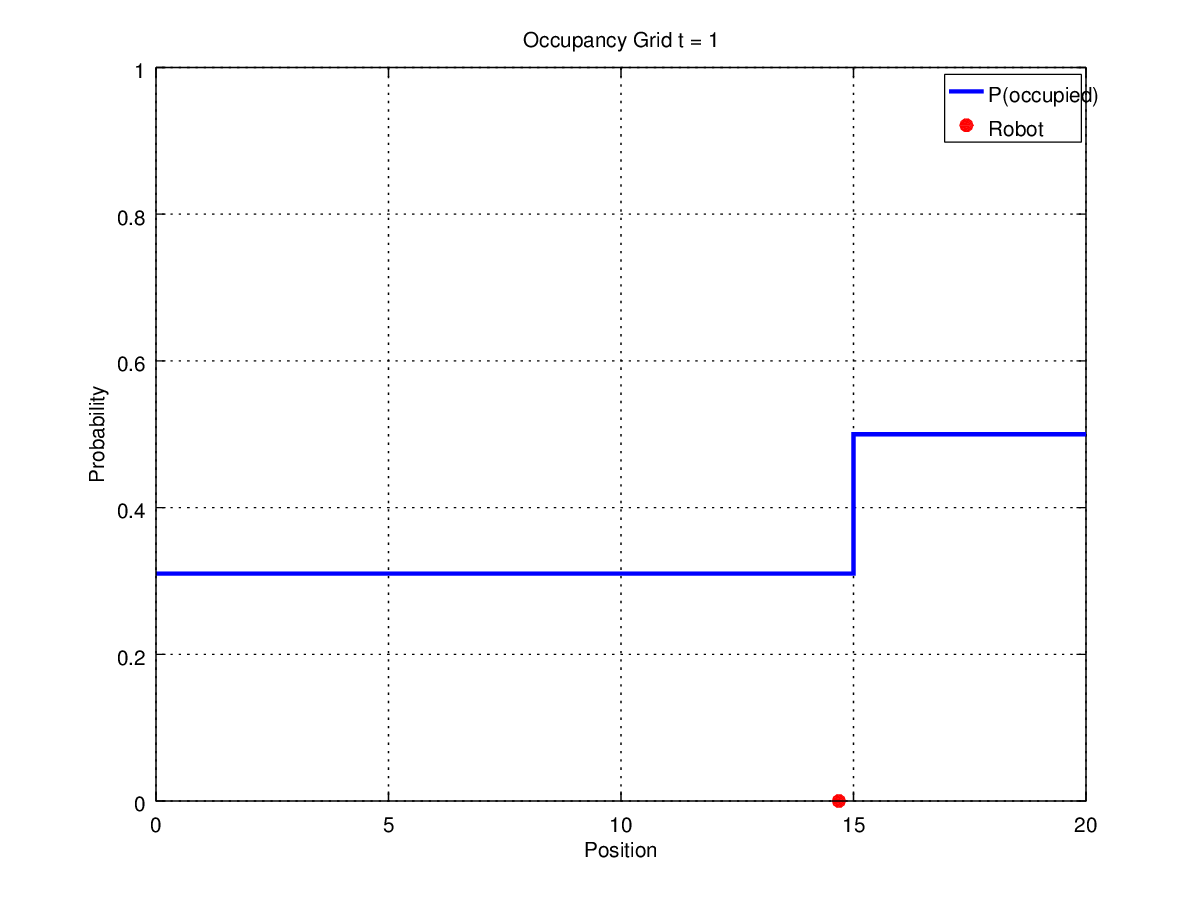
\includegraphics[width=\linewidth,height=2in]{occupgrid/occupgrid1.png}
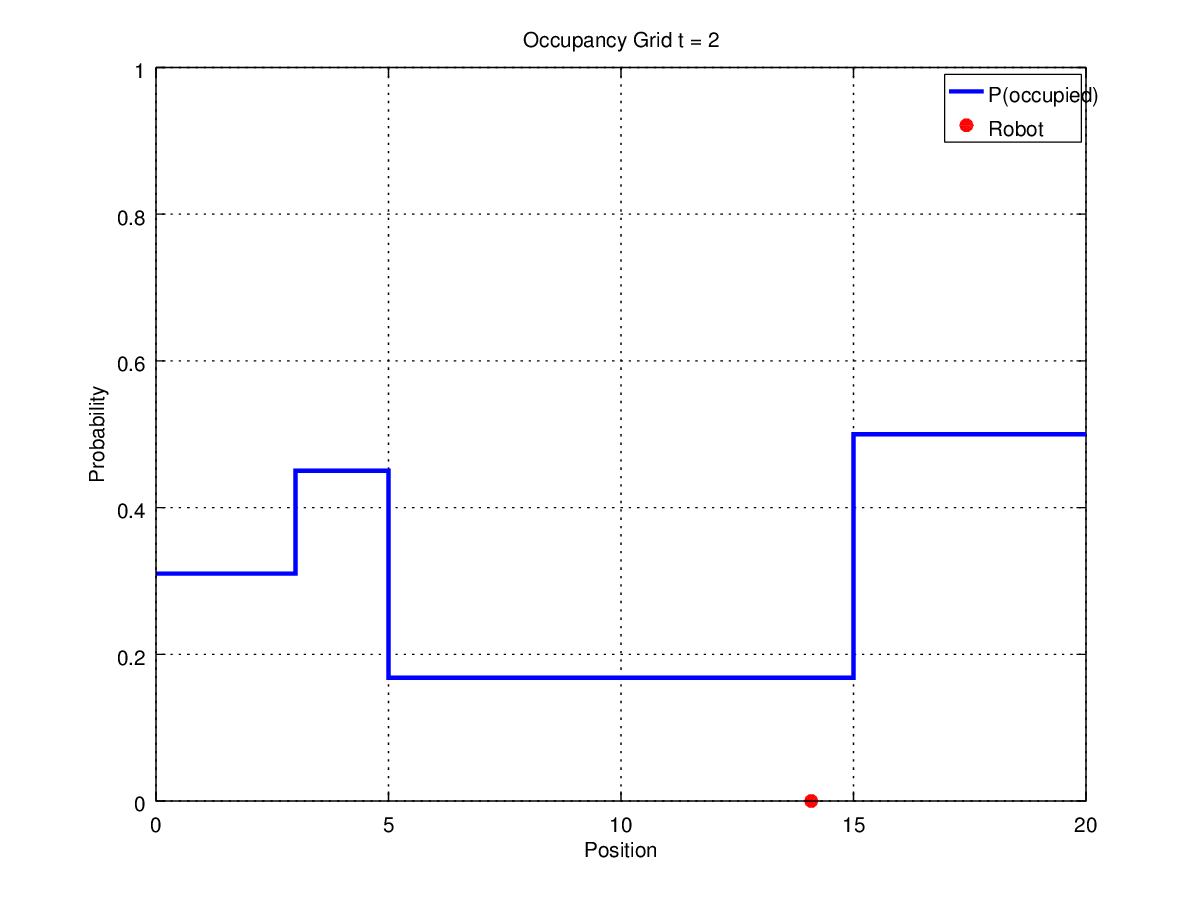
\includegraphics[width=\linewidth,height=2in]{occupgrid/occupgrid2.png}
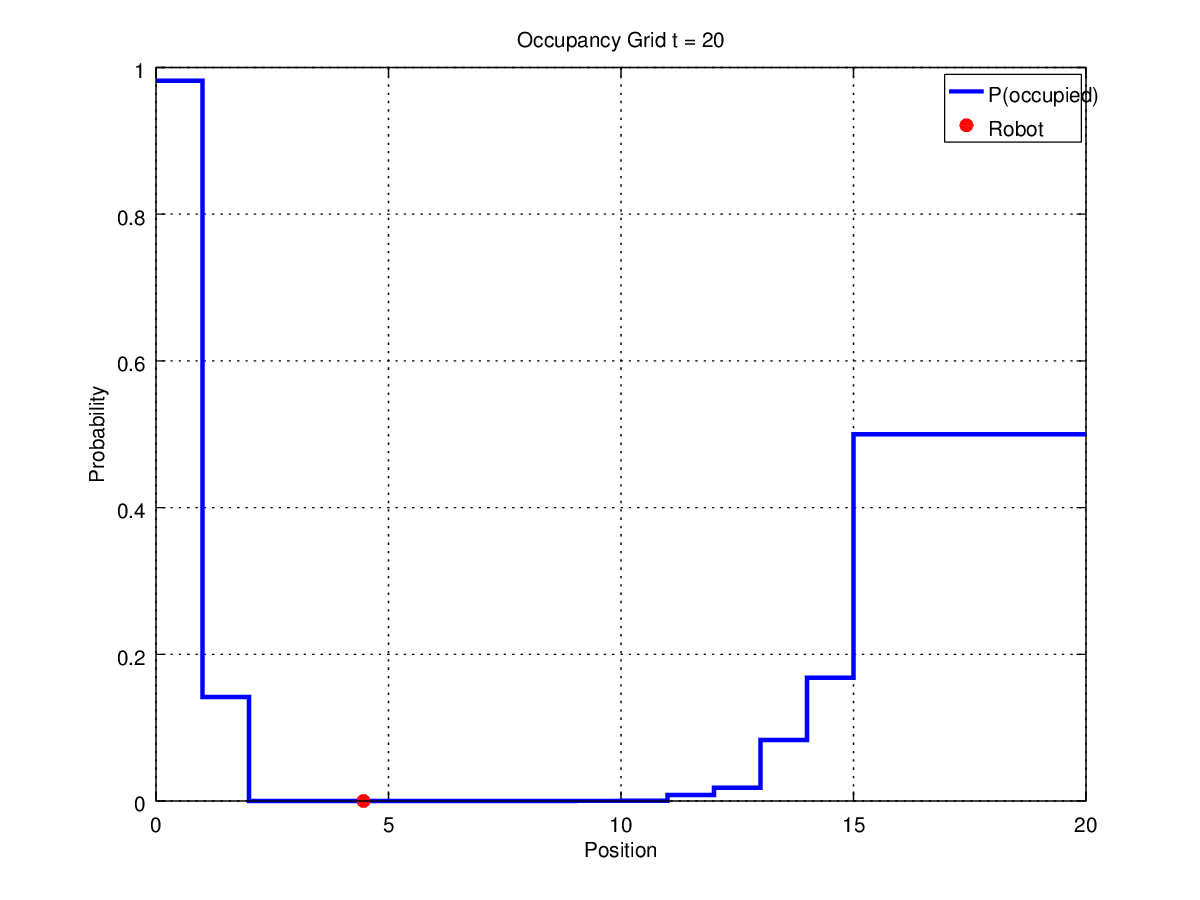
\includegraphics[width=\linewidth,height=2in]{occupgrid/occupgrid20.png}
\caption{An example of occupancy grids for a 1D robot with a range sensor moving towards a wall at position 0.  The red dot is the actual robot position.  The blue curve is the occupancy grid probability.}
\label{fig:occupgrid}
\end{figure}

\section{Recommendation}

For planar mobile robot mapping, a recommended approach is to use occupancy grids for the world map representation with SLAM.  Occupancy grids do not require sophisticated data association as with landmarks and work with simple sensing such as range sensors.  The particular SLAM algorithm could either be a variant of FastSLAM or GraphSLAM.

\section{Experiments}

\begin{align}
x_t &= x_{t-1} + v_l \cos (\theta_{t-1}) \\
y_t &= y_{t-1} + v_l \sin (\theta_{t-1}) \\
\theta_t &= \theta_t + \omega
\end{align}

\begin{align}
v_l &= r \frac{\omega_L + \omega_R}{2}
\end{align}

\appendix

\section{Derivations}

\subsection{Recursive Bayes Filter}

The derivation of the recursive Bayes filter follows from Bayes's Rule, exploiting conditional indepenence assumptions, and some algebra:
\begin{align}
p(s_t, M | z_{1:t}, u_{1:t})  &=  \frac{1}{A} p(z_t | s_t, M, z_{1:t-1}, u_{1:t}) p(s_t, M | z_{1:t-1}, u_{1:t}) \\
&=  \frac{1}{A} p(z_t | s_t, M) p(s_t, M | z_{1:t-1}, u_{1:t}) \\
&=  \frac{1}{A} p(z_t | s_t, M) \int p(s_t, M | s_{t-1}, z_{1:t-1}, u_{1:t}) p(s_{t-1} | z_{1:t-1}, u_{1:t}) ds_{t-1} \\
&=  \frac{1}{A} p(z_t | s_t, M) \int p(s_t | M, s_{t-1}, z_{1:t-1}, u_{1:t}) p(M | s_{t-1}, z_{1:t-1}, u_{1:t}) p(s_{t-1} | z_{1:t-1}, u_{1:t}) ds_{t-1} \\
&=  \frac{1}{A} p(z_t | s_t, M) \int p(s_t | s_{t-1}, u_t) p(s_{t-1}, M | z_{1:t-1}, u_{1:t}) ds_{t-1} \\
&=  \frac{1}{A} p(z_t | s_t, M) \int p(s_t | s_{t-1}, u_t) p(s_{t-1}, M | z_{1:t-1}, u_{1:t-1}) ds_{t-1}.
\end{align}
The last line in the equations above show the recursion in which the current probability distribution $p(s_t, M | z_{1:t}, u_{1:t})$ is written in terms of the product of the measurement distribution $p(z_t | s_t, M)$ and an integral involving the previous probability distribution $p(s_{t-1}, M | z_{1:t-1}, u_{1:t-1})$ and the robot motion model $p(s_t | s_{t-1}, u_t)$.

\subsection{Occupancy Grid Update}

The derivation of the occupancy grid cell log odds update follows from specializing the recursive Bayes filter to this case of a binary cell state:
\begin{align}
p(m_i | z_{1:t}, s_{1:t}) &= \frac{p(z_t | m_i, z_{1:t-1}, s_{1:t}) p(m_i | z_{1:t-1}, s_{1:t})}{p(z_t | z_{1:t-1}, s_{1:t})} \\
&= \frac{p(z_t | m_i, s_{1:t}) p(m_i | z_{1:t-1}, s_{1:t})}{p(z_t | z_{1:t-1}, s_{1:t})} \\
&= \frac{p(m_i | z_t, s_{1:t}) p(z_t | s_{1:t}) p(m_i | z_{1:t-1}, s_{1:t})}{p(m_i | s_{1:t})p(z_t | z_{1:t-1}, s_{1:t})}.
\end{align}
To simplify, we take the log odds:
\begin{align}
L_{i, t} &= \log \frac{p(m_i = 1 | z_{1:t}, s_{1:t})}{p(m_i = 0| z_{1:t}, s_{1:t})} \\
&= \log \frac{p(m_i = 1 | z_t, s_{1:t}) p(m_i = 1 | z_{1:t-1}, s_{1:t}) p(m_i = 0 | s_{1:t})}{p(m_i = 0 | z_t, s_{1:t}) p(m_i = 0 | z_{1:t-1}, s_{1:t}) p(m_i = 1 | s_{1:t})} \\
&= \log \frac{p(m_i = 1 | z_t, s_{1:t}) p(m_i = 1 | z_{1:t-1}, s_{1:t}) [1 - p(m_i = 1 | s_{1:t})]}{[1 - p(m_i = 1 | z_t, s_{1:t})] [1 - p(m_i = 1 | z_{1:t-1}, s_{1:t})] p(m_i = 1 | s_{1:t})} \\
&= \log \frac{p(m_i = 1 | z_t, s_{1:t})}{1 - p(m_i = 1 | z_t, s_{1:t})} + \log \frac{p(m_i = 1 | z_{1:t-1}, s_{1:t})}{1 - p(m_i = 1 | z_{1:t-1}, s_{1:t})} + \log \frac{1 - p(m_i = 1 | s_{1:t})}{p(m_i = 1 | s_{1:t})} \\
&= L_{i, t-1} + \log \frac{p(m_i = 1 | z_t, s_{1:t})}{1 - p(m_i = 1 | z_t, s_{1:t})} - L_0.
\end{align}
Note again the recursion from the previous log odds $L_{i, t-1}$ and the measurement model $p(m_i = 1 | z_t, s_{1:t})$ to the current log odds, $L_{i, t}$.

\section{Background}

\subsection{Bayes}

Bayes's Rule is simple.  Starting with the joint probability distribution of the relevant random variables, we expand it in two ways:
\begin{equation}
p(s_t , z_t) = p(z_t | s_t) p(s_t) = p(s_t | z_t) p(z_t).
\end{equation}
Equating the two expansions and re-arranging we obtain the rule:
\begin{equation}
p(s_t | z_t) = \frac{p(z_t | s_t) p(s_t)}{p(z_t)}.
\end{equation}
The utility of Bayes's Rule is that it allows one to factor a probability distribution, $p(s_t | z_t)$ into a product of two terms, $p(z_t | s_t)$ and $p(s_t)$, which may lead to easier computation.  For example, $p(z_t | s_t)$ may represent the distribution of the sensor measurement $z_t$ given the robot state $s_t$.

\subsection{Kalman Filter} \label{sec:kalman}

The Kalman filter is a recursive Bayes filter assuming linear-Gaussian models:
\begin{align}
p(s_t | s_{t-1}, u_t) &= N(A_t s_{t-1} + B_t u_t, R_t), \\
p(z_t | s_t) &= N(C_t s_t,  Q_t), \\
p(s_0) &= N(\mu_0, \Sigma_0).
\end{align}
The above equations show that the initial probability distribution of the state is Gaussian.  Also, the measurement model is Gaussian noise added to a linear function of the state.  Finally, the state transition distribution is also Gaussian on a linear function of the previous state and the control.

The Kalman filter model involves mainly keeping track of the Gaussian mean and covariance, $\mu_t$ and $\Sigma_t$, which fully characterize the Gaussian distribution of the state over time.  Given the linear-Gaussian model, the recursive Bayes filter (Kalman) updates are as follows:
\begin{align}
\hat{\mu}_t &= A_t \mu_{t-1} + B_t u_t, \\
\hat{\Sigma}_t &= A_t \Sigma_{t-1} A_t^T + R_t, \\
K_t &= \hat{\Sigma}_t C_t^T (C_t \hat{\Sigma}_t C_t^T + Q_t)^{-1}, \\
\mu_t &= \hat{\mu}_t + K_t (z_t - C_t \hat{\mu}_t), \\
\Sigma_t &= (I - K_t C_t) \hat{\Sigma}_t.
\end{align}

Consider  a 1D example of a linear robot facing a wall such that the robot can only translate perpendicular to the wall.  The robot has a range sensor which gives a noisy distance to the wall where the noise decreases with distance.  For simplicity, let the wall be at position 0, so that the range $z_t$ is a noisy measurement of the robot position $s_t$.  The Kalman filter model can be written as follows:
\begin{align}
p(s_t | s_{t-1}, u_t) &= N(s_{t-1} + u_t, r^2) \\
p(z_t | s_t) &= N(s_t,  q^2) \\
p(s_0) &= N(\mu_0, \sigma^2_0)
\end{align}
where $\mu_0$ is the mean of the initial position, and $u_t$ is the robot translation.  In this case, the Kalman updates are simple and intuitive:
\begin{align}
\hat{\mu}_t &= \mu_{t-1} + u_t, \\
\hat{\sigma}^2_t &= \sigma^2_{t-1} + r^2, \\
k_t &= \frac{\hat{\sigma}^2_t}{\hat{\sigma}^2_t + q^2_t}, \\
\mu_t &= \hat{\mu}_t + k_t (z_t - \hat{\mu}_t), \\
\sigma^2_t &= (1 - k_t) \hat{\sigma}^2_t.
\end{align}
The predicted mean is the previous mean plus the control.  The predicted variance is the previous variance plus the variance from the control.  The Kalman gain balances the predicted variance and the measurement variance.  The posterior mean adds a weighted adjustment to the predicted mean.  The posterior variance is a scaled version of the predicted variance depending on the Kalman gain.  Figure \ref{fig:kalman} shows an example run of the Kalman filter.  Initially the uncertainty is high and the prediction is poor, but as the robot moves towards the wpwd
cdall the range measurements are more accurate and the confidence in the estimated position increases.

\begin{figure}
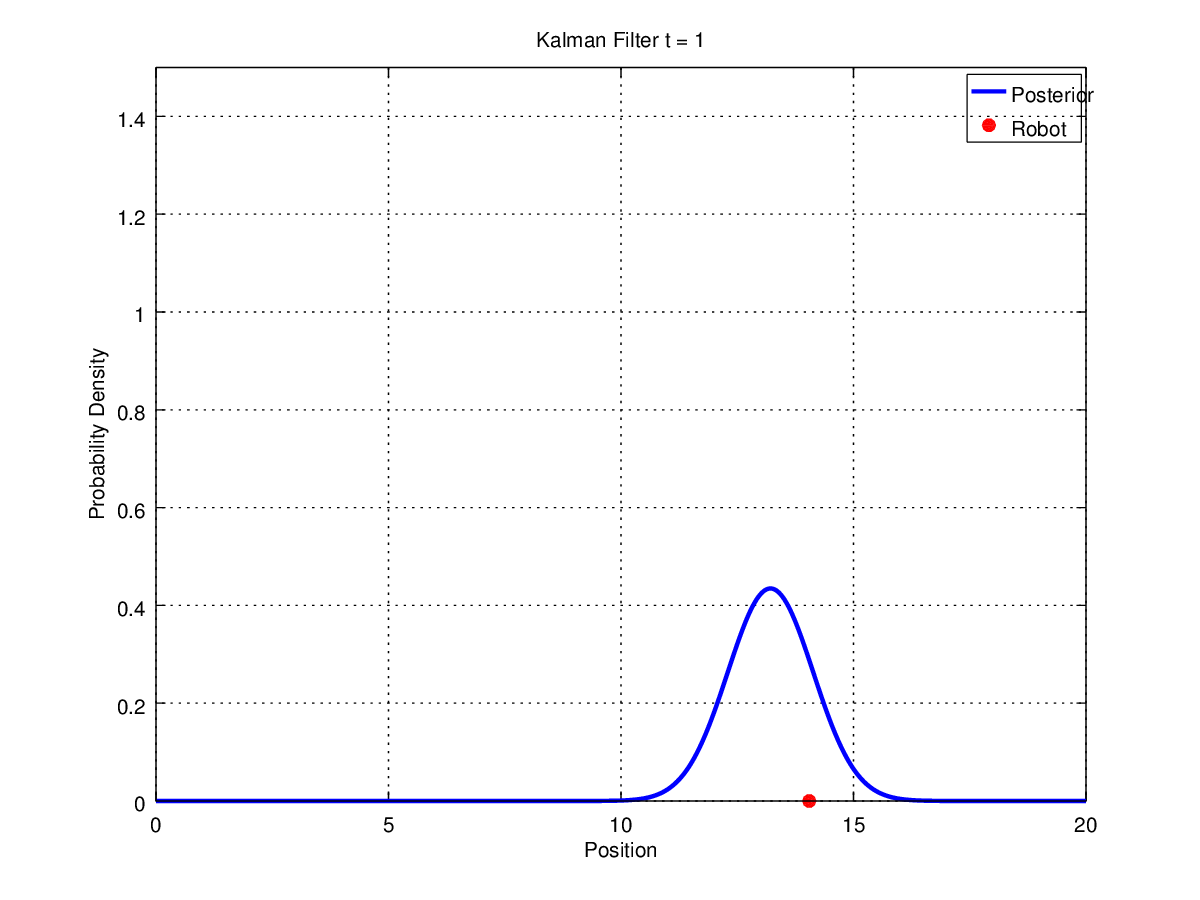
\includegraphics[width=\linewidth,height=2.25in]{kalman/kalman1.png}
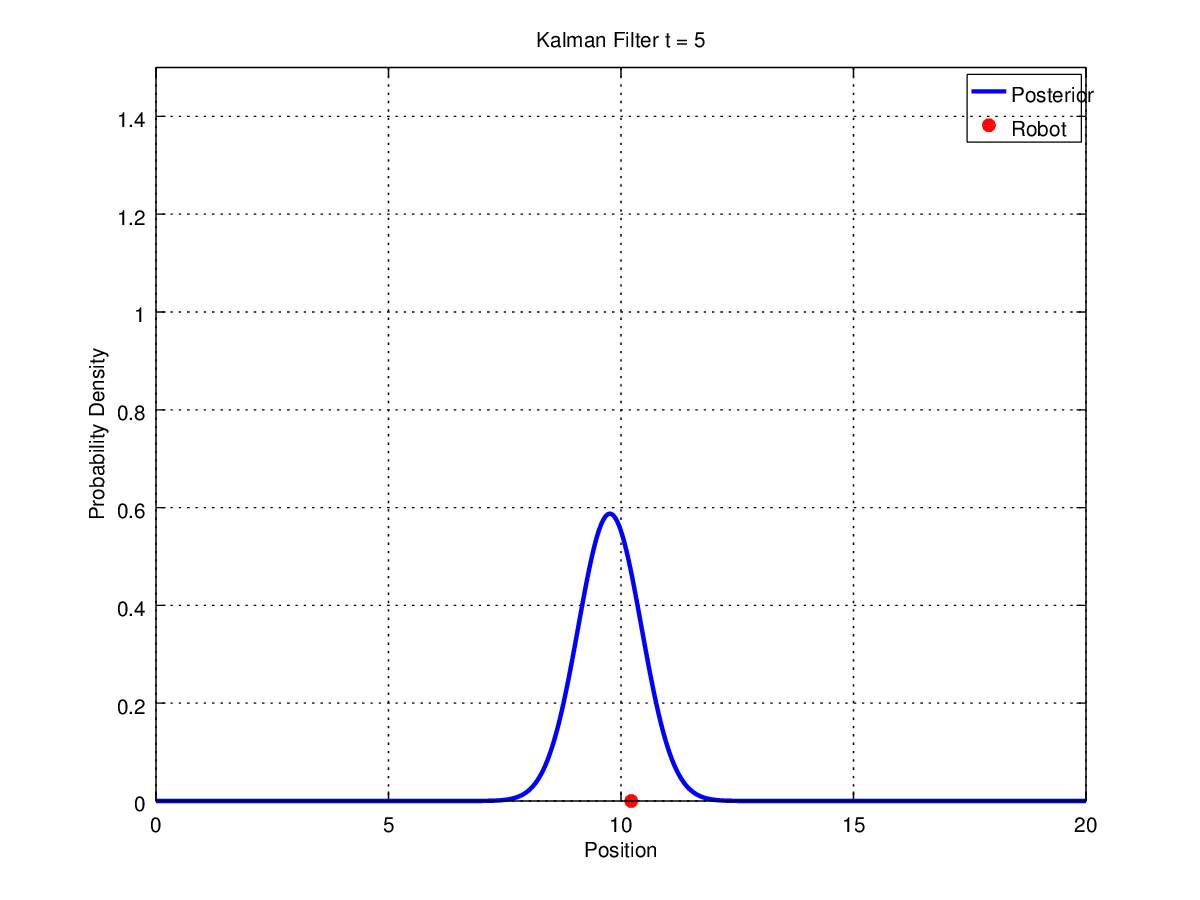
\includegraphics[width=\linewidth,height=2.25in]{kalman/kalman5.png}
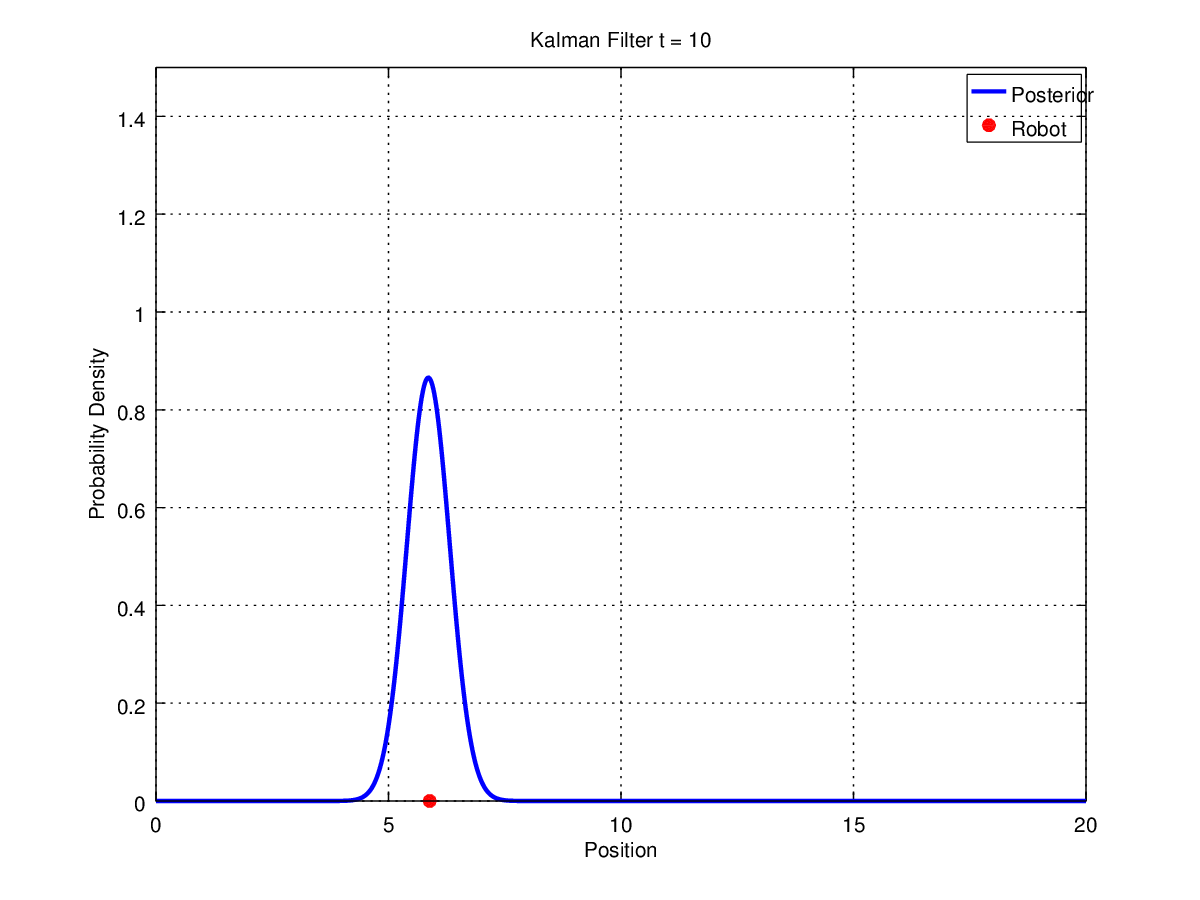
\includegraphics[width=\linewidth,height=2.25in]{kalman/kalman10.png}
\caption{An example of Kalman filtering the position of 1D robot with a range sensor moving towards a wall at position 0.  The red dot is the actual robot position.  The blue curve is the Kalman posterior distribution of the robot position.}
\label{fig:kalman}
\end{figure}

\subsection{Extended Kalman Filter}

The extended Kalman filter (EKF) is an extension of the Kalman filter to nonlinear state transition and measurement models:
\begin{align}
s_t &= g(u_t, s_{t-1}) + v_t, \\
z_t &= h(s_t) + w_t,
\end{align}
where $v_t$ and $w_t$ are the state and measurement noise, with zero mean and covariance $R_t$ and $Q_t$, respectively.  The EKF approximates the posterior probability distributions as Gaussian by linearizing around the mean via Taylor expansion of the nonlinear models:
\begin{align}
g(u_t, s_{t-1}) &\approx g(u_t, \mu_{t-1}) + G_t(s_{t-1} - \mu_{t-1}), \\
h(s_t) &\approx h(\hat{\mu}_t) + H_t(s_t - \hat{\mu}_t),
\end{align}
where
\begin{align}
G_t &= \frac{\partial g(u_t, s_{t-1})}{\partial s_{t-1}}(\mu_{t-1}), \\
H_t &= \frac{\partial h(s_t)}{\partial s_t}(\hat{\mu}_t).
\end{align}
Thus the EKF updates are almost identical to the Kalman updates except that $G_t$ and $H_t$ take the place of ($A_t$, $B_t$) and $C_t$, respectively.

\subsection{Particle Filter}

The particle filter implements the recursive Bayes filter by representing the posterior probability distribution $p(s_t | z_{1:t}, u_{1:t})$ with a sample of particles, $x_{t, 1}, x_{t, 2}, \ldots, x_{t, n}$.  Assume that the current particles were drawn from the previous posterior $p(s_{t-1} | z_{1:t-1}, u_{1:t-1})$.  First it draws temporary particles based on the robot motion model:
\begin{equation}
\hat{x}_{t, i} \sim p(x_t | x_{t-1, i}, u_t).
\end{equation}
Then the measurement is incorporated by computing a weight for the temporary particles:
\begin{equation}
w_{i, i} = p(z_t | \hat{x}_{t, i}).
\end{equation}
Finally new particles are drawn according to the weights.  This completes the recursion so that the new particles represent a sample from the posterior distribution:
\begin{equation}
x_{t, i} \sim p(s_t | z_{1:t}, u_{1:t}).
\end{equation}

The particle filter works by using importance sampling which is a way to generate a sample from one probability distribution $p$ by a weighted drawing of a sample from another distribution $q$.  Consider computing the expectation under $p$ of a function $f$:
\begin{align}
E_p[f(x)] &= \int_x p(x) f(x) dx \\
&= \int_x  q(x) \frac{p(x)}{q(x)} f(x) dx \\
&= \int_x  q(x) w(x) f(x) dx \\
&= E_q[w(x)f(x)] \\
&\approx \frac{1}{n} \sum_{i=1}^n w(x_i) f(x_i)
\end{align}
where
\begin{equation}
w(x) = \frac{p(x)}{q(x)}.
\end{equation}

The particle filter algorithm is simple and can approximate probability distributions beyond Gaussians.  However, for an accurate approximation, the number of particles $n$ may need to be large, which increases the computational burden.

\bibliographystyle{plain}
\bibliography{main}
\nocite{*}

\end{document}
